%GiG
\documentclass{beamer} 
\usetheme{Copenhagen}
\setbeamertemplate{navigation symbols}{}
\setbeamertemplate{headline}{}
\DeclareMathOperator*{\argmax}{arg\,max}

\usepackage{hyperref}


\definecolor{azure}{rgb}{0.0, 0.5, 1.0}
%\newcommand{\tblue}[1]{\textcolor{blue}{#1}}
\newcommand{\tblue}[1]{{\Large {\textcolor{azure}{#1}}}}
\newcommand{\thblue}[1]{{\Huge {\textcolor{azure}{#1}}}}
\newcommand{\hred}[1]{{\textcolor{red}{#1}}}
\newcommand{\furl}[1]{{\footnote{\url{#1}}}}

\newcommand{\mypause}{\pause}
%\newcommand{\mypause}{}

\title[Saravanan Thirumuruganathan] 
{Lecture 7: Decision Trees}

\author[CSE 5334] 
{Instructor: Saravanan Thirumuruganathan}

\date[] 

\begin{document}


\begin{frame}
  \titlepage
\end{frame}

%\begin{frame}{Outline}
%  \tableofcontents
%  % You might wish to add the option [pausesections]
%\end{frame}

\section{Outline}

\begin{frame}
\frametitle {Outline}
\begin{enumerate}
\item Geometric Perspective of Classification
\item Decision Trees
\end{enumerate}
\end{frame}


%\begin{frame}{In-Class Quizzes}
%\begin{itemize}
%\item {\Large {\bf URL:}} {\LARGE \bf \url{http://m.socrative.com/}} 
%\item {\Large {\bf Room Name:} {\LARGE \bf 4f2bb99e}}
%\end{itemize}
%\end{frame}


\section{Geometric Perspective of Classification}
\begin{frame}{} 
    \begin{center}
        \thblue{Geometric Perspective of Classification}
    \end{center}
\end{frame}

\begin{frame}{Perspective of Classification}
    \begin{itemize}
        \item Algorithmic
        \item Geometric 
        \item Probabilistic
        \item $\ldots$
    \end{itemize}
\end{frame}

\begin{frame}{Geometric Perspective of Classification}
    \begin{itemize}
        \item Gives some intuition for model selection
        \item Understand the distribution of data
        \item Understand the expressiveness and limitations of various classifiers
    \end{itemize}
\end{frame}

\begin{frame}{Feature Space\footnote{DMA Book}}
    \begin{center}
        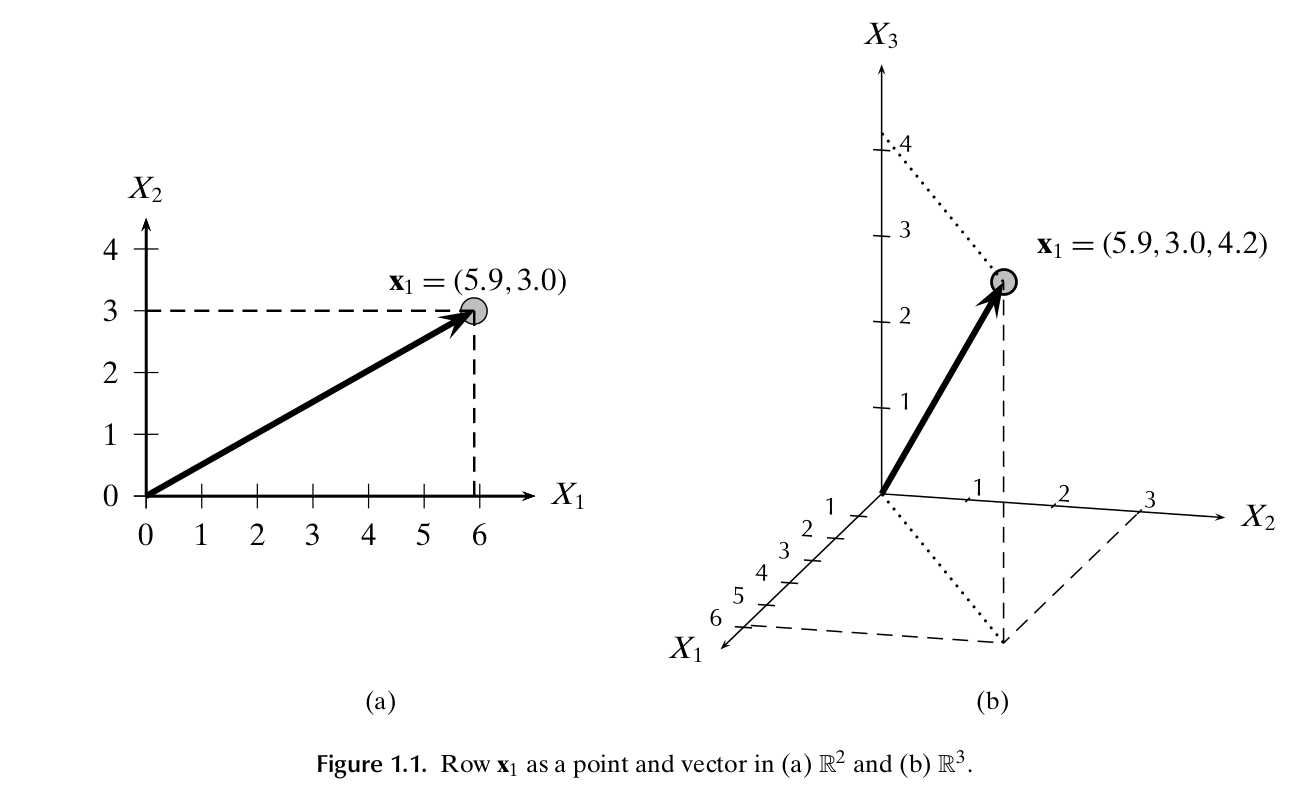
\includegraphics[scale=0.15]{geometricView.png}
    \end{center}
    \begin{itemize}
        \item {\bf Feature Vector:} $d$-dimensional vector of features describing the object
        \item {\bf Feature Space:} The vector space associated with feature vectors
    \end{itemize}
\end{frame}

\begin{frame}{Feature Space in Classification}
    \begin{center}
        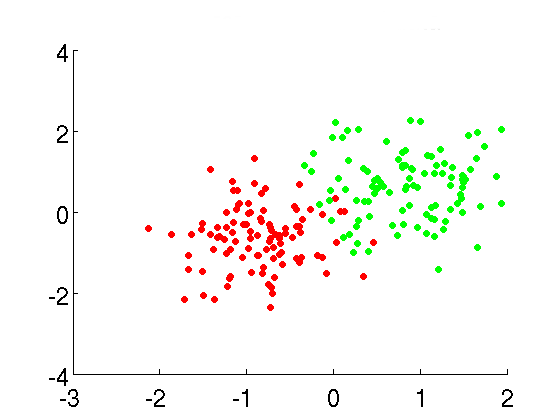
\includegraphics[scale=0.5]{featureSpace.png}
    \end{center}
\end{frame}

\begin{frame}{Geometric Perspective of Classification}
    \begin{itemize}
        \item {\bf Decision Region:} A partition of feature space such that all feature vectors in it are assigned to same class.
        \item {\bf Decision Boundary:} Boundaries between neighboring decision regions
    \end{itemize}
\end{frame}


\begin{frame}{Geometric Perspective of Classification}
    \begin{itemize}
        \item Objective of a classifier is to {\em approximate} the ``real'' decision boundary as much as possible 
        \item Most classification algorithm has specific expressiveness and limitations
        \item If they align, then classifier does a good approximation
    \end{itemize}
\end{frame}

\begin{frame}{Linear Decision Boundary}
    \begin{center}
        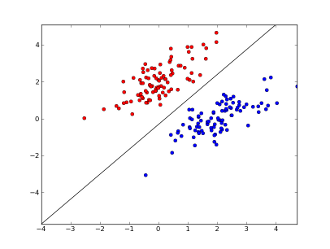
\includegraphics[scale=0.75]{linearDecisionBoundary.png}
    \end{center}
\end{frame}
\begin{frame}{Piecewise Linear Decision Boundary\footnote{ISLR Book}}
    \begin{center}
        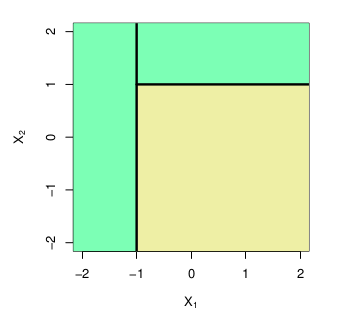
\includegraphics[scale=0.6]{piecewiseLinearDecisionBoundary.png}
    \end{center}
\end{frame}
\begin{frame}{Quadratic Decision Boundary\footnote{Figshare.com}}
    \begin{center}
        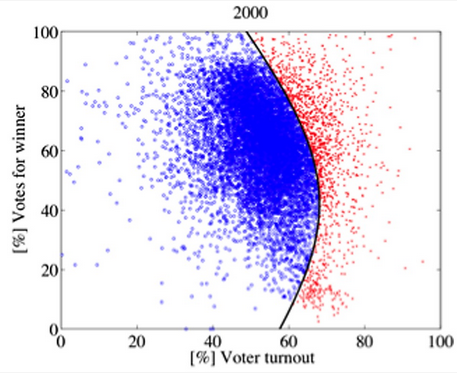
\includegraphics[scale=0.5]{quadraticDecisionBoundary.png}
    \end{center}
\end{frame}
\begin{frame}{Non-linear Decision Boundary\footnote{ISLR Book}}
    \begin{center}
        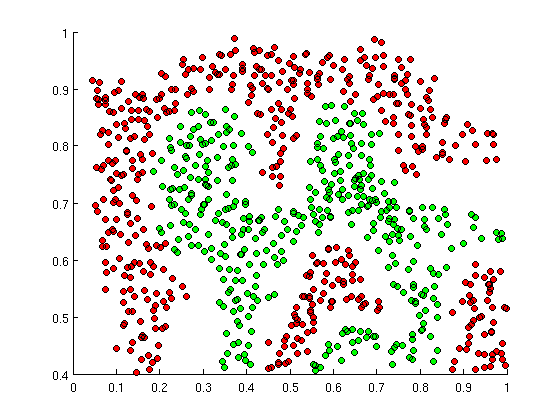
\includegraphics[scale=0.5]{nonlinearDecisionBoundary.png}
    \end{center}
\end{frame}
\begin{frame}{Complex Decision Boundary\footnote{ISLR Book}}
    \begin{center}
        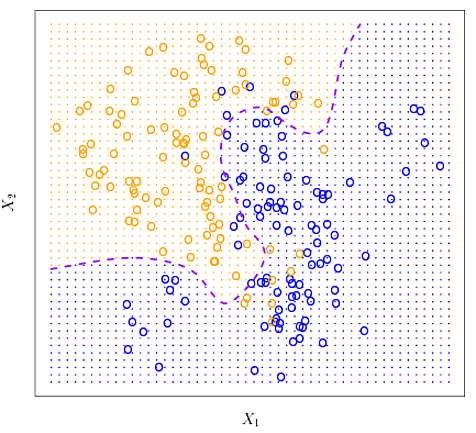
\includegraphics[scale=0.5]{complexDecisionBoundary.png}
    \end{center}
\end{frame}

\begin{frame}{Classifier Selection Tips}
    \begin{itemize}
        \item If decision boundary is linear, most {\em linear} classifiers will do well
        \item If decision boundary is non-linear, we sometimes have to use kernels 
        \item If decision boundary is piece-wise, decision trees can do well
        \item If decision boundary is too complex, $k$-NN might be a good choice
    \end{itemize}
\end{frame}

\begin{frame}{$k$-NN Decision Boundary\footnote{ISLR Book}}
    \begin{center}
        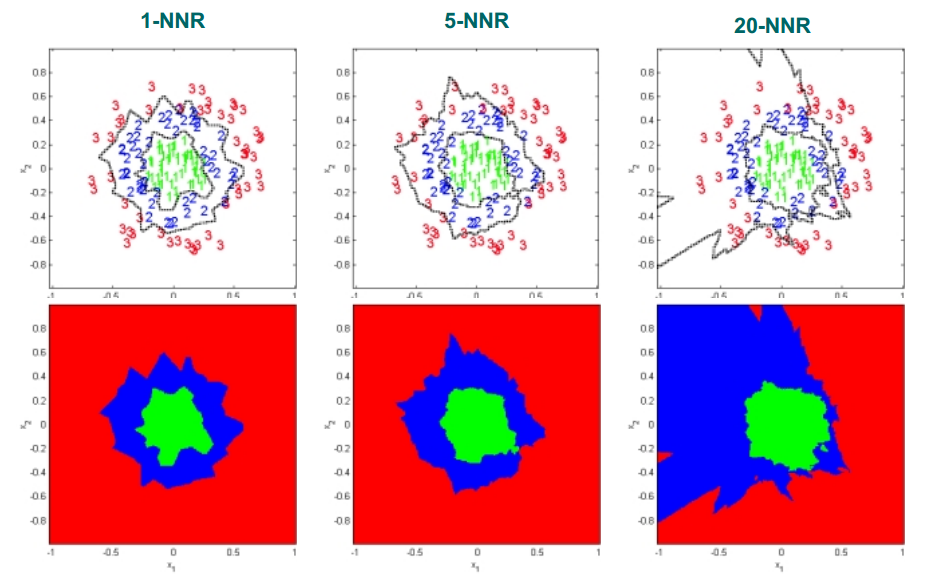
\includegraphics[scale=0.2]{kNNVaringK.png}
    \end{center}

    \begin{itemize}
       \item Asymptotically Consistent: With infinite training data and large enough $k$, $k$-NN approaches the best possible classifier (Bayes Optimal)
       \item With infinite training data and large enough $k$, $k$-NN could approximate most possible decision boundaries
    \end{itemize}
\end{frame}

\section{Decision Trees}
\begin{frame}{} 
    \begin{center}
        \thblue{Decision Trees}
    \end{center}
\end{frame}

\begin{frame}{Strategies for Classifiers}
    \begin{itemize}
        \item {\bf Parametric Models: } Makes some assumption about data distribution such as density and often use explicit probability models
        \item {\bf Non-parametric Models: } No prior assumption of data and determine decision boundaries directly.
        \begin{itemize}
            \item $k$-NN
            \item Decision tree
        \end{itemize}
    \end{itemize}
\end{frame}

\begin{frame}{Tree\furl{http://statweb.stanford.edu/~lpekelis/talks/13_datafest_cart_talk.pdf}}
    \begin{center}
        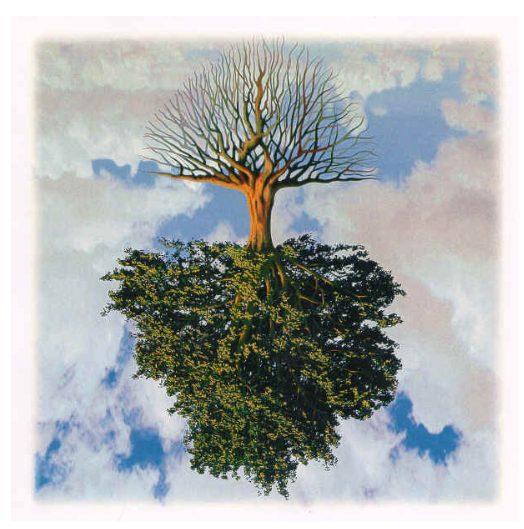
\includegraphics[scale=0.4]{tree.png}
    \end{center}
\end{frame}
\begin{frame}{Binary Decision Tree\furl{http://statweb.stanford.edu/~lpekelis/talks/13_datafest_cart_talk.pdf}}
    \begin{center}
        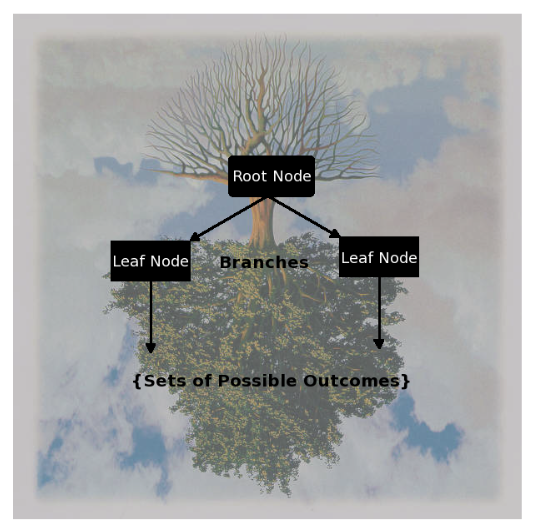
\includegraphics[scale=0.4]{binaryDTree.png}
    \end{center}
\end{frame}
\begin{frame}{20 Question Intuition\furl{http://www.idiap.ch/~fleuret/files/EE613/EE613-slides-6.pdf}}
    \begin{center}
        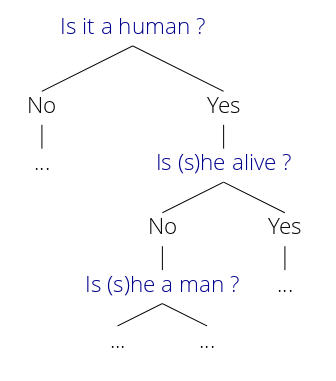
\includegraphics[scale=0.4]{20QAsDTree.png}
    \end{center}
\end{frame}
\begin{frame}{Decision Tree for Selfie Stick\footnote{The Oatmeal Comics}}
    \begin{center}
        
\includegraphics[scale=0.30]{selfie_stick.jpg}
    \end{center}
\end{frame}

\begin{frame}{Decision Trees and Rules\furl{http://artint.info/slides/ch07/lect3.pdf}}
    \begin{center}
        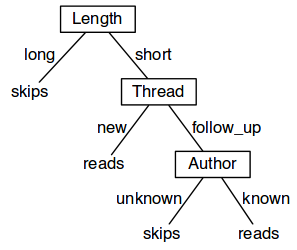
\includegraphics[scale=0.50]{egDTrees.png}
    \end{center}
\end{frame}
\begin{frame}{Decision Trees and Rules\furl{http://artint.info/slides/ch07/lect3.pdf}}
    \begin{columns}
        \column{0.58\linewidth}
            \begin{itemize}
                \item long $\rightarrow$ skips
                \item short $\wedge$ new $\rightarrow$ reads 
                \item short $\wedge$ follow Up $\wedge$ known $\rightarrow$ reads 
                \item short $\wedge$ follow Up $\wedge$ unknown $\rightarrow$ skips 
            \end{itemize}
            
        \column{0.38\linewidth}
            \centering
            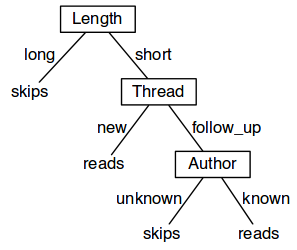
\includegraphics[scale=0.40]{egDTrees.png}
    \end{columns}
\end{frame}

\begin{frame}{Building Decision Trees Intuition\furl{http://spark-summit.org/wp-content/uploads/2014/07/Scalable-Distributed-Decision-Trees-in-Spark-Made-Das-Sparks-Talwalkar.pdf}}
\begin{center}
    \begin{table}
        \begin{tabular}{| c | c | c |}
            \hline
            {\bf Horsepower} & {\bf Weight} & \textcolor{blue}{{\bf Mileage}} \\ \hline
                95 & low & low \\ \hline
                90 & low & low \\ \hline
                70 & low & high \\ \hline
                86 & low & high \\ \hline
                76 & high & low \\ \hline
                88 & high & low \\ \hline
        \end{tabular}
        \caption{Car Mileage Prediction from 1971}
    \end{table}
\end{center}
\end{frame}
\begin{frame}{Building Decision Trees Intuition}
\begin{center}
    \begin{table}
        \begin{tabular}{| c | c | c |}
            \hline
            {\bf Horsepower} & {\bf Weight} & \textcolor{blue}{{\bf Mileage}} \\ \hline
                95 & low & low \\ \hline
                90 & low & low \\ \hline
                70 & low & high \\ \hline
                86 & low & high \\ \hline
                \textcolor{green}{76} & \textcolor{green}{high} & \textcolor{green}{low} \\ \hline
                \textcolor{green}{88} & \textcolor{green}{high} & \textcolor{green}{low} \\ \hline
        \end{tabular}
        \caption{Car Mileage Prediction from 1971}
    \end{table}
\end{center}
\end{frame}
\begin{frame}{Building Decision Trees Intuition}
    \begin{center}
        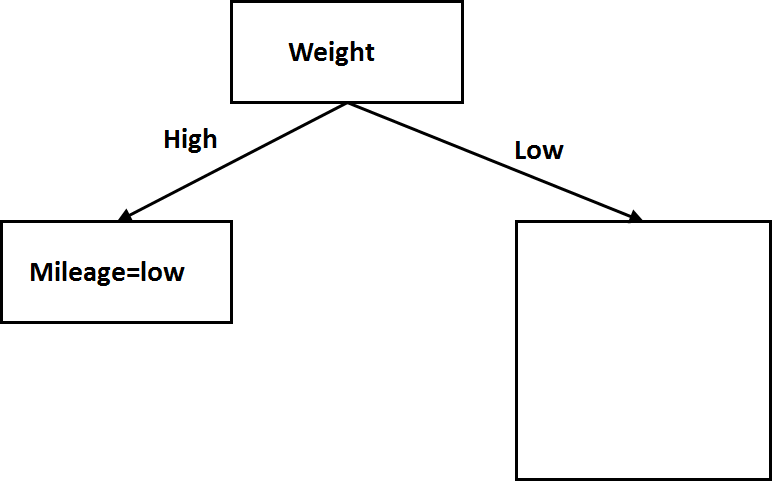
\includegraphics[scale=0.5]{dTreeEg1.png}
    \end{center}
\end{frame}
\begin{frame}{Building Decision Trees Intuition}
\begin{center}
    \begin{table}
        \begin{tabular}{| c | c | c |}
            \hline
            {\bf Horsepower} & {\bf Weight} & \textcolor{blue}{{\bf Mileage}} \\ \hline
                95 & low & low \\ \hline
                90 & low & low \\ \hline
                70 & low & high \\ \hline
                86 & low & high \\ \hline
        \end{tabular}
        \caption{Car Mileage Prediction from 1971}
    \end{table}
\end{center}
\end{frame}
\begin{frame}{Building Decision Trees Intuition}
    \begin{center}
        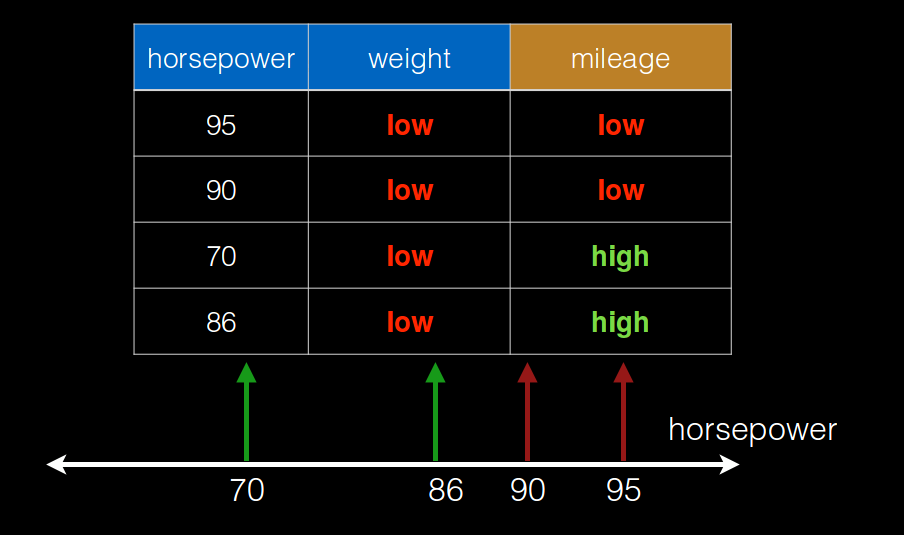
\includegraphics[scale=0.3]{dTreeEg2.png}
    \end{center}
\end{frame}
\begin{frame}{Building Decision Trees Intuition}
    \begin{center}
        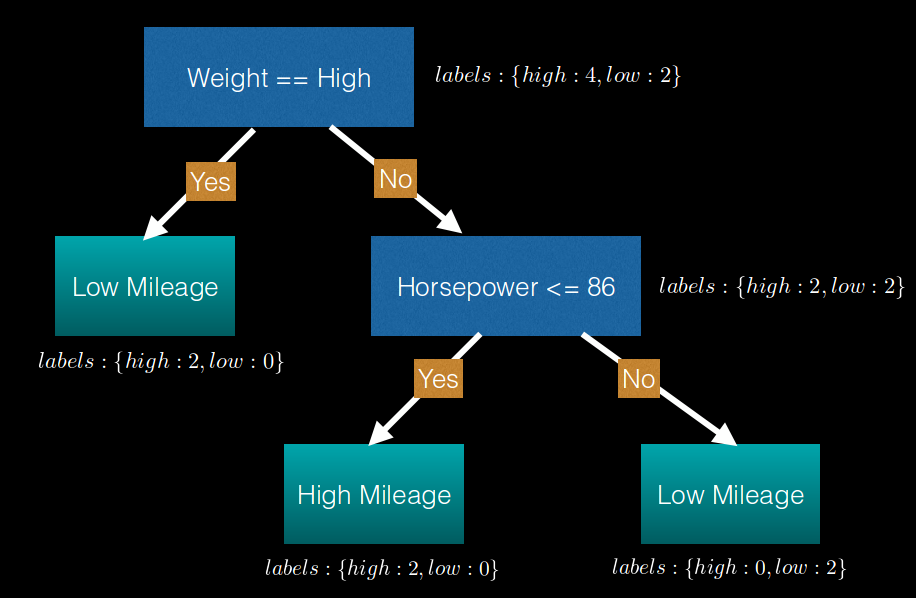
\includegraphics[scale=0.3]{dTreeEg3.png}
    \end{center}
\end{frame}
\begin{frame}{Building Decision Trees Intuition}

    {\bf Prediction:}
    \begin{center}
        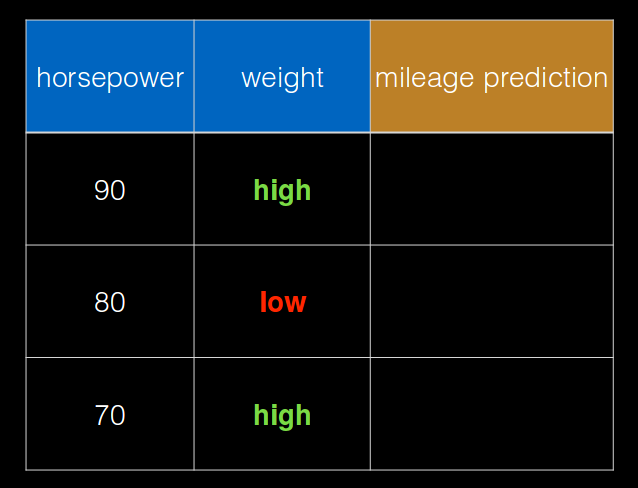
\includegraphics[scale=0.3]{dTreeEg4.png}
    \end{center}
\end{frame}
\begin{frame}{Building Decision Trees Intuition}

    {\bf Prediction:}
    \begin{center}
        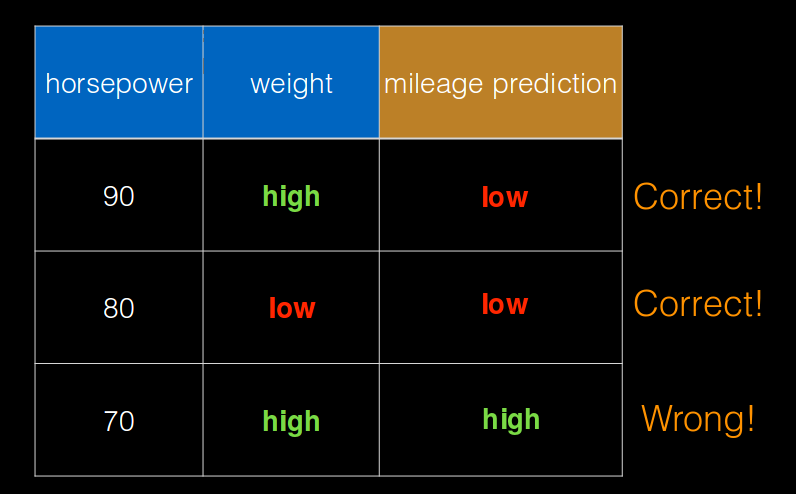
\includegraphics[scale=0.3]{dTreeEg5.png}
    \end{center}
\end{frame}


\section{Learning Decision Trees}
\begin{frame}{} 
    \begin{center}
        \thblue{Learning Decision Trees}
    \end{center}
\end{frame}

\begin{frame}{Decision Trees}
    \begin{itemize}
        \item Defined by a {\bf hierarchy} of rules (in form of a tree)
            \begin{center}
                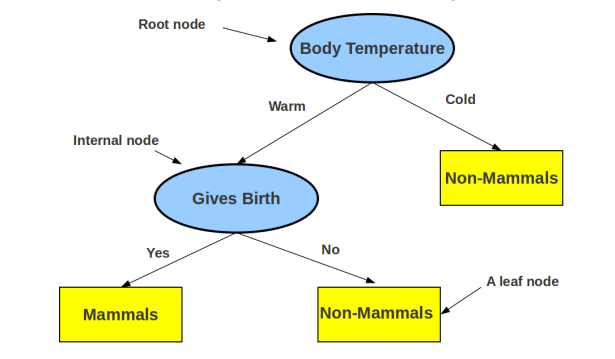
\includegraphics[scale=0.3]{dTreeExpl.png}
            \end{center}
        \item Rules form the internal nodes of the tree (topmost internal node = root)
        \item Each rule (internal node) tests the value of some property the data
        \item Leaf nodes make the prediction
    \end{itemize}
\end{frame}


\begin{frame}{Decision Tree Learning}

    {\bf Objective:} 
    \begin{itemize}
        \item Use the training data to construct a good decision tree
        \item Use the constructed Decision tree to predict labels for test inputs
    \end{itemize}
\end{frame}

\begin{frame}{Decision Tree Learning}
    \begin{itemize}
        \item Identifying the region (blue or green) a point lies in
        \begin{itemize}
            \item A classification problem (blue vs green)
            \item Each input has 2 features: co-ordinates $\{x_1, x_2\}$ in the 2D plane
        \end{itemize}
        \item Once learned, the decision tree can be used to predict the region (blue/green) of a new test point
    \end{itemize}
\end{frame}

\begin{frame}{Decision Tree Learning}
    \begin{center}
        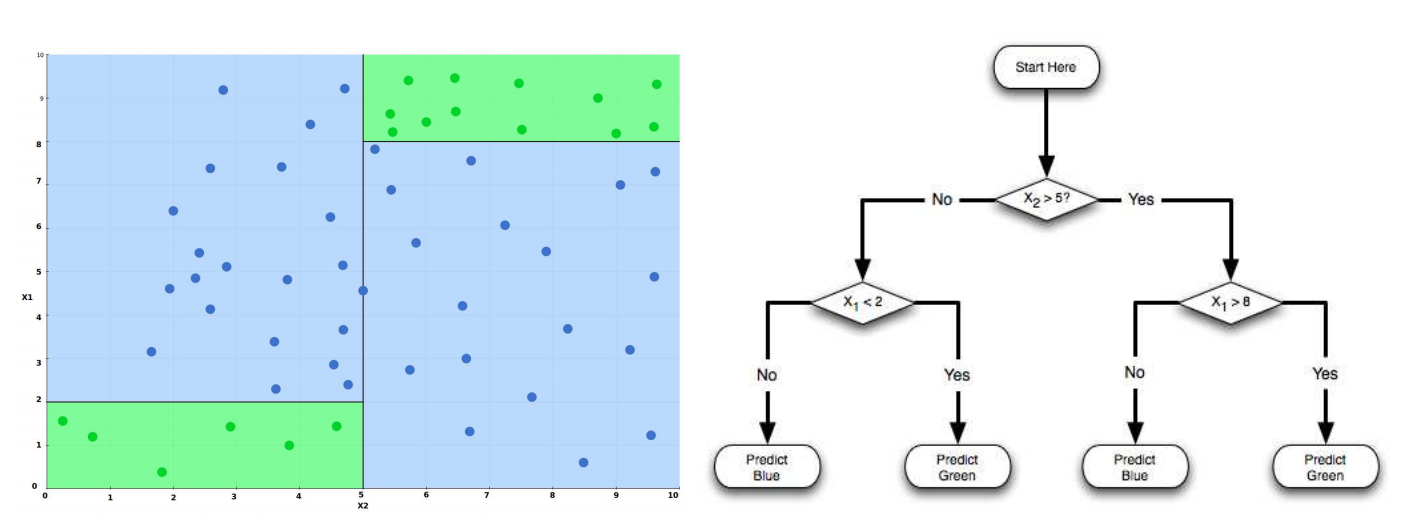
\includegraphics[scale=0.23]{dTreeLearning1.png}
    \end{center}
\end{frame}

\begin{frame}{Expressiveness of Decision Trees}
    \begin{columns}
        \column{0.48\linewidth}
            \centering
            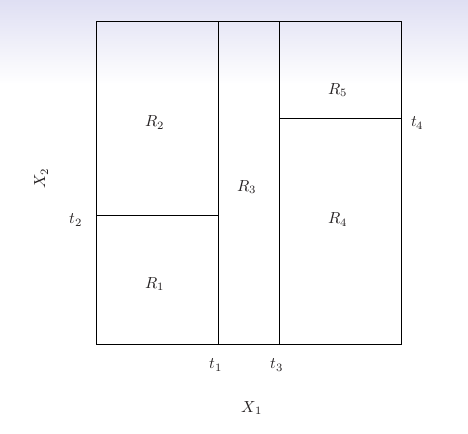
\includegraphics[scale=0.40]{dTreeExpressiveness1.png}
            
        \column{0.48\linewidth}
            \centering
            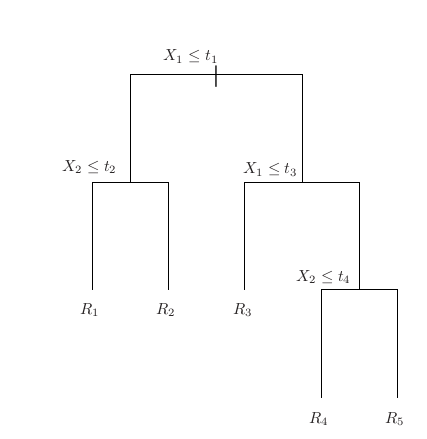
\includegraphics[scale=0.40]{dTreeExpressiveness2.png}
    \end{columns}
\end{frame}

\begin{frame}{Expressiveness of Decision Trees}
    \begin{itemize}
        \item Decision tree divides feature space into {\bf axis-parallel} rectangles
        \item Each rectangle is labelled with one of the $C$ classes
        \item Any partition of feature space by recursive binary splitting can be simulated by Decision Trees
    \end{itemize}
\end{frame}

\begin{frame}{Expressiveness of Decision Trees}
    \begin{columns}
        \column{0.48\linewidth}
            \centering
            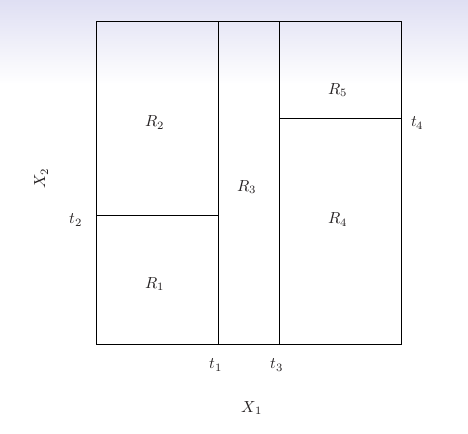
\includegraphics[scale=0.36]{dTreeExpressiveness1.png}
            
        \column{0.48\linewidth}
            \centering
            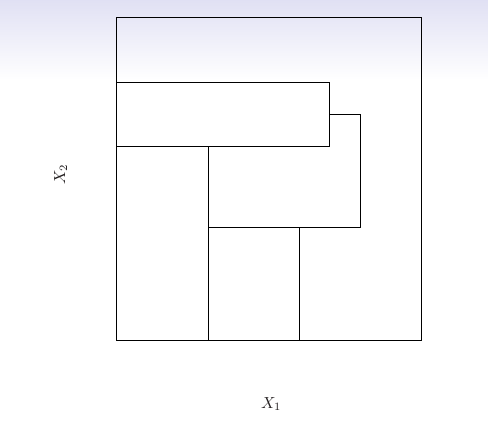
\includegraphics[scale=0.40]{dTreeExpressiveness3.png}
    \end{columns}

    \pause Feature space on left can be simulated by Decision tree but not the one on right.
\end{frame}

\begin{frame}{Expressiveness of Decision Tree}
    \begin{columns}
        \column{0.48\linewidth}
            \begin{itemize}
                \item Can express any logical function on input attributes
                \item Can express {\bf any} boolean function
                \item For boolean functions, path to leaf gives truth table row
                \item Could require exponentially many nodes
                \item $cyl=3 \vee (cyl=4 \wedge (maker=asia \vee maker=europe)) \vee \ldots $
            \end{itemize}
            
        \column{0.48\linewidth}
            \centering
            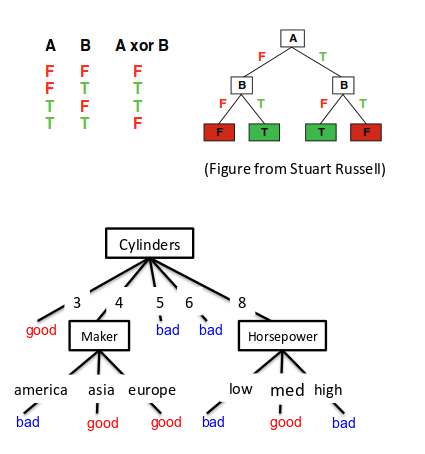
\includegraphics[scale=0.30]{dTreeFunctions.png}
    \end{columns}
\end{frame}

\begin{frame}{Hypothesis Space}
    \begin{itemize}
        \item Exponential search space wrt set of attributes
        \item If there are $d$ boolean attributes, then the search space has $2^{2^d}$ trees
        \begin{itemize}
            \item If $d=6$, then it is approximately $2 \times 10^{18}$
            \item If there are $d$ boolean attributes, each truth table has $2^d$ rows
            \item Hence there must be $2^{2^d}$ truth tables that can take all possible variations 
        \end{itemize}
        \item NP-Complete to find optimal decision tree
        \item Idea: Use greedy approach to find a locally optimal tree
    \end{itemize}
\end{frame}

\begin{frame}{Decision Tree Learning Algorithms}
    \begin{itemize}
        \item 1966: Hunt and colleagues from Psychology developed first known algorithm for human concept learning
        \item 1977: Breiman, Friedman and others from Statistics developed CART
        \item 1979: Quinlan developed proto-ID3
        \item 1986: Quinlan published ID3 paper
        \item 1993: Quinlan's updated algorithm C4.5
        \item 1980's and 90's: Improvements for handling noise, continuous attributes, missing data, non-axis parallel DTs, better heuristics for pruning, overfitting, combining DTs
    \end{itemize}
\end{frame}

\begin{frame}{Decision Tree Learning Algorithms}
    
    Main Loop:
    \begin{enumerate}
        \item Let $A$ be the ``best'' decision attribute for next node
        \item Assign $A$ as decision attribute for node
        \item For each value of $A$, create a new descendent of node
        \item Sort training examples to leaf nodes
        \item If training examples are perfectly classified, then STOP else iterate over leaf nodes
    \end{enumerate}
\end{frame}


\begin{frame}{Decision Tree Learning}
    \begin{itemize}
        \item Greedy Approach: Build tree, top-down by choosing one attribute at a time
        \item Choices are locally optimal and may or may not be globally optimal 
        \item Major issues
        \begin{itemize}
            \item Selecting the next attribute
            \item Determining termination condition
        \end{itemize}
    \end{itemize}
\end{frame}


\begin{frame}{Termination Condition}

    Stop expanding a node further when: \pause
    \begin{itemize}
        \item It consist of examples all having the same label 
        \item Or we run out of features to test!
    \end{itemize}
\end{frame}


\begin{frame}{Recursive Algorithm for Learning Decision Trees}
    \begin{center}
        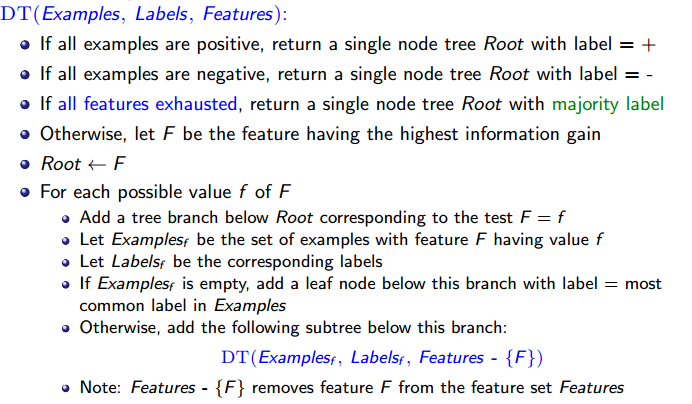
\includegraphics[scale=0.4]{dTreeLearningAlgo.png}
    \end{center}
\end{frame}


\begin{frame}{}
    \begin{itemize}
        \item 
    \end{itemize}
\end{frame}


\begin{frame}{}
    \begin{itemize}
        \item 
    \end{itemize}
\end{frame}


\begin{frame}{}
    \begin{itemize}
        \item 
    \end{itemize}
\end{frame}


\begin{frame}{}
    \begin{itemize}
        \item 
    \end{itemize}
\end{frame}


\begin{frame}{}
    \begin{itemize}
        \item 
    \end{itemize}
\end{frame}


\begin{frame}{}
    \begin{itemize}
        \item 
    \end{itemize}
\end{frame}


\section{Summary}
\begin{frame}{Summary}

\tblue{Major Concepts:}
\begin{itemize}
    \item Geometric interpretation of Classification
    \item Decision trees
\end{itemize}
\end{frame}

\begin{frame}{Slide Material References}
\begin{itemize}
    \item Slides from ISLR book
    \item Slides by Piyush Rai
    \item Slides for Chapter 4 from ``Introduction to Data Mining'' book by Tan, Steinbach, Kumar
    \item See also the footnotes
\end{itemize}
\end{frame}


\end{document}

